%=================================================================
\section{USE Of BASIC TOOLS AND WEBSITES}\label{sec-intro}
By learning the LaTeX Use Introduction shared by the team, I successfully completed the installation of TeX Live and downloaded the team's package from CTAN.Appendices A, B, and the first four chapters were studied and run with Texworks.\par
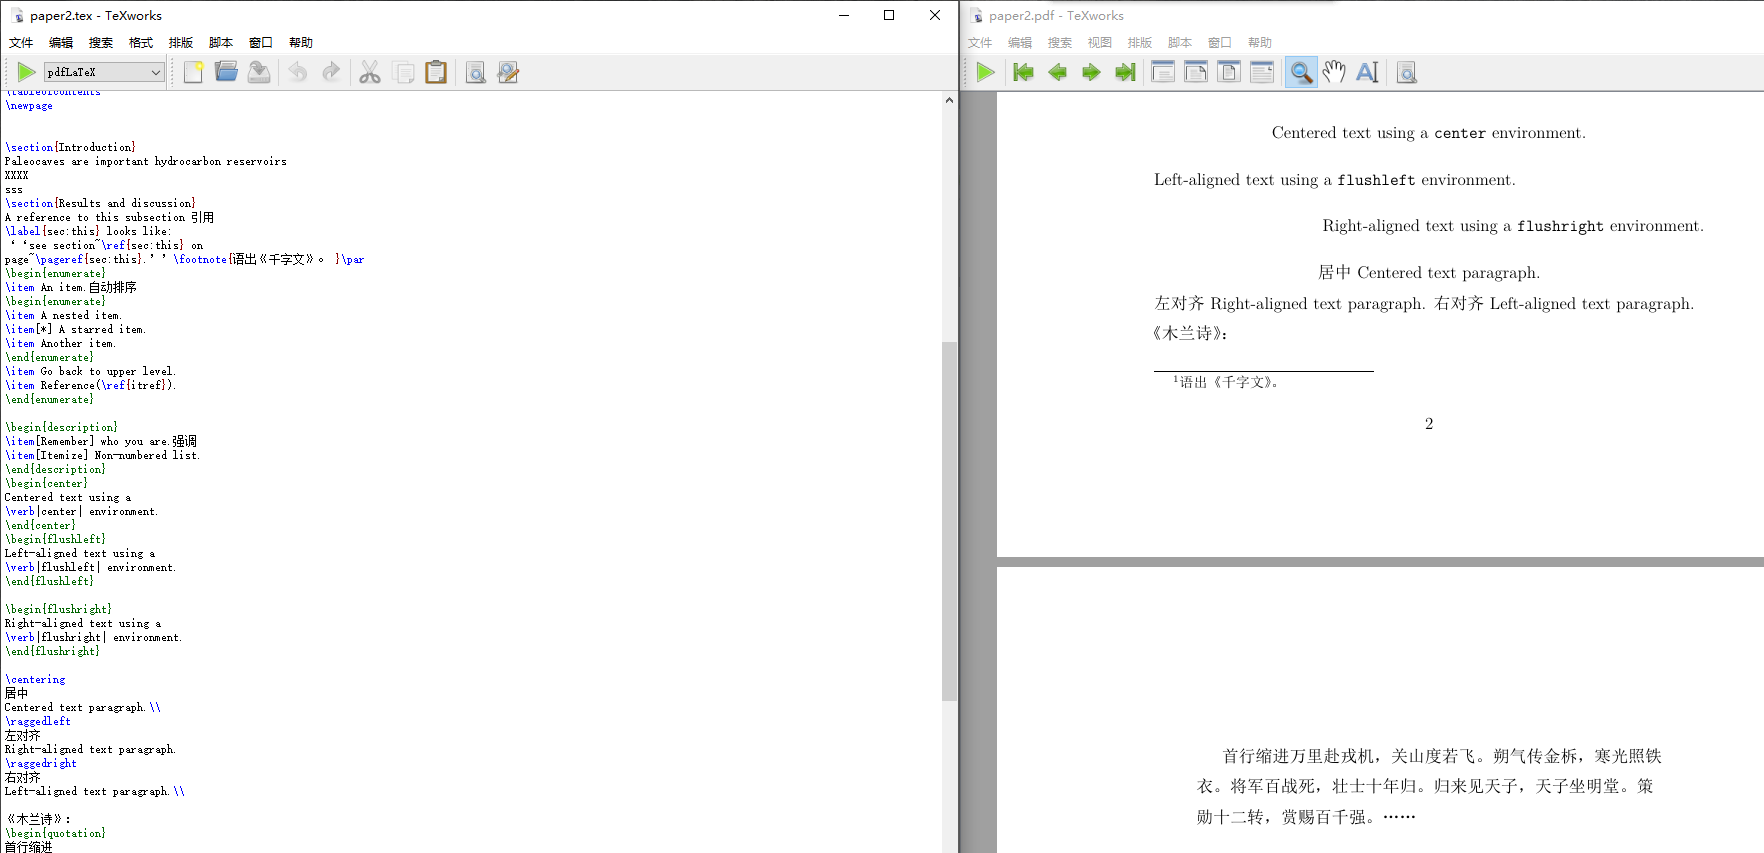
\includegraphics[scale=0.25]{Latex2}\par
Team recommended that we use Notion as a commonly used notebook app. By referring to the template used by our team, I have made a learning plan for one week. Currently, I am not sure about my learning speed, so I cannot plan my KOR yet.\par
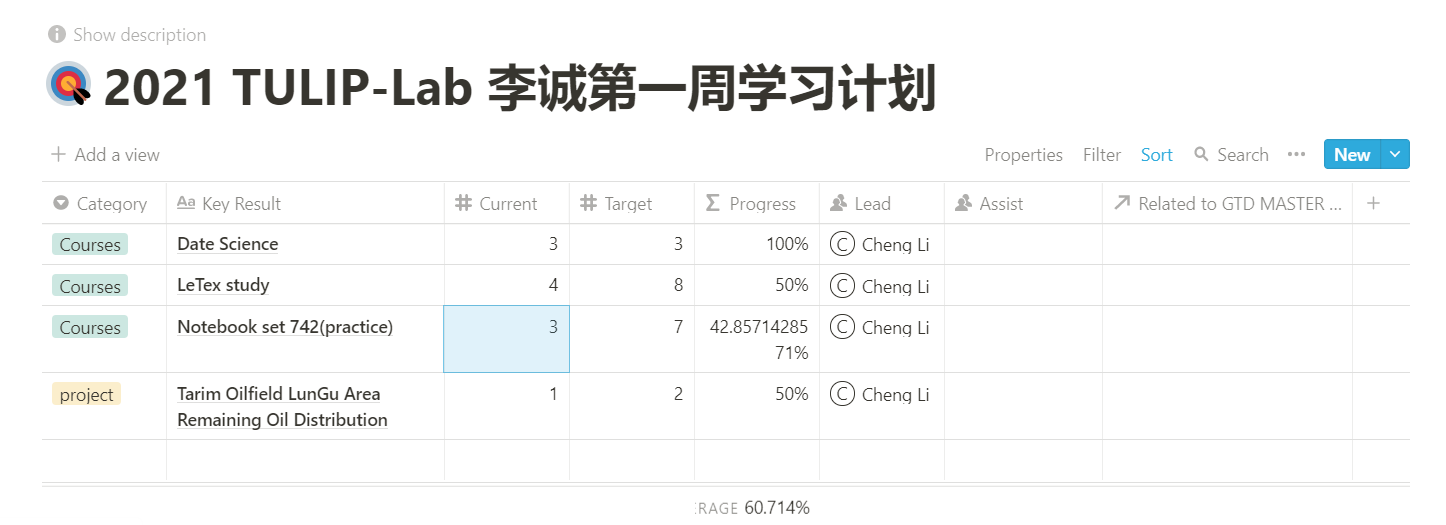
\includegraphics[scale=0.3]{notion}\par
In addition, I created a lot of accounts this week, like Kaggle, Anaconda, Databricks...\par
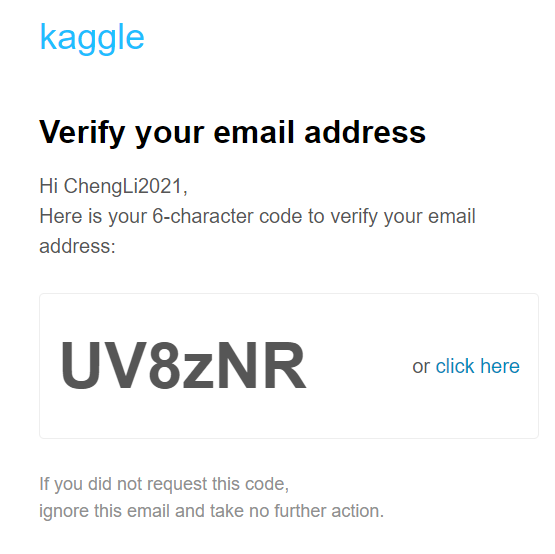
\includegraphics[scale=0.3]{kaggle}\par

\section{Date Science} \label{sec-preliminaries}
On the date of li gang, a professor at the science three quarters after class, I think of my biggest harvest is I think the door is professional and I am currently major can be very good fusion, my major is currently faced with a lot of oil and gas well production or geophysical data in combination with geological theory instruction to summarize regularity, this step in processing data, machine learning or data analysis technology can achieve very good effect or a better efficiency.\par
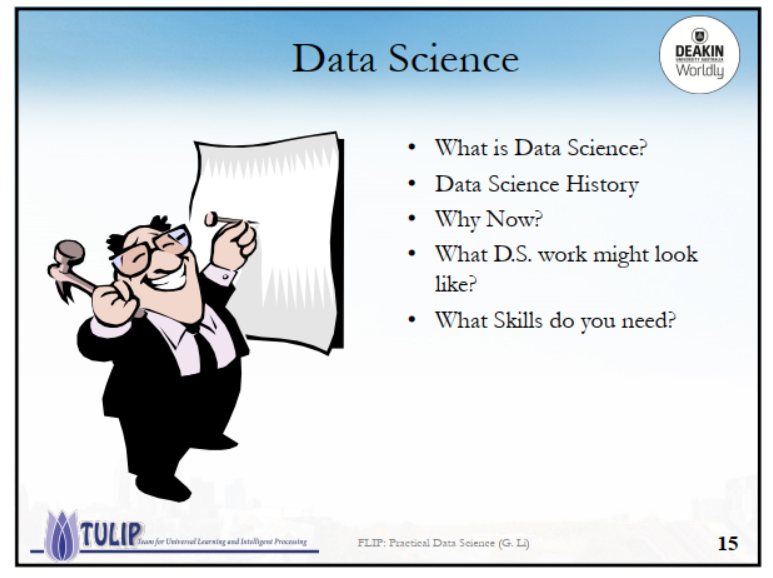
\includegraphics[scale=0.4]{date science1}\par
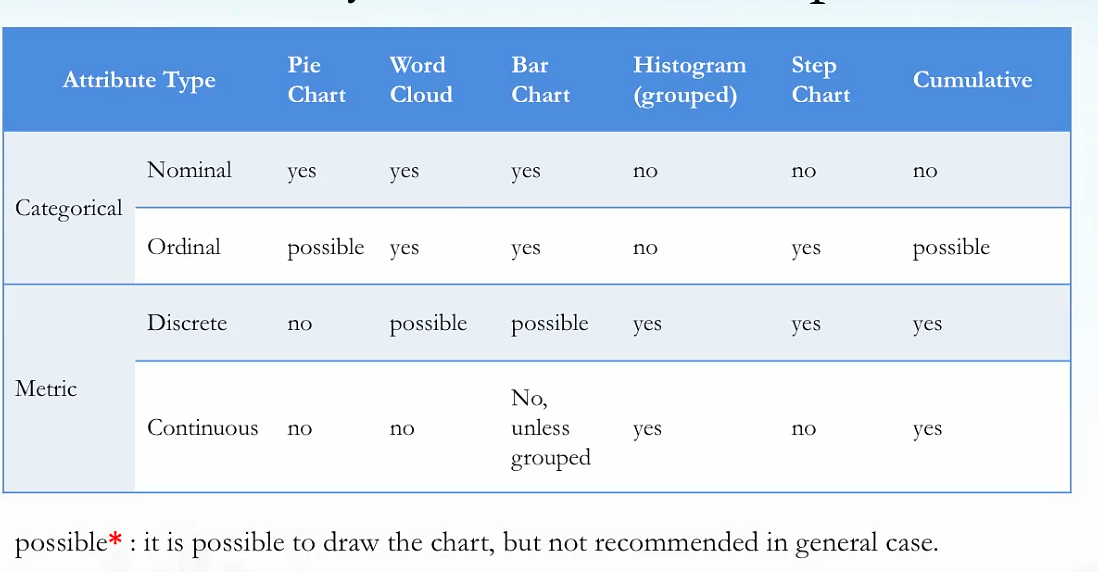
\includegraphics[scale=0.3]{date science2}\par
  \par
  \par

\section{QUESTION} \label{sec-method}





